\section{Background}
Energy consumption is ever increasing and our current electrical grid is outdated, as it is unable to handle the more dynamic production and consumption of power we have today.
There is also an increasing generation of renewable energy (e.g. wind and solar energy), but optimal use of this is limited by our current electrical grid.
As it is now, renewable sources are often shut down if they are producing more than can be consumed.
On the other hand, during periods with little renewable power, more expensive and environmentally unsafe sources are used.
Most net suppliers only support very simple tariffs with one fixed price, or a single division of prices, throughout the day \cite{smart_meter_survey}.

The statements above has led to an increased focus on energy usage, with optimizations of the electrical grid as a high priority, which is why by 2022 all\footnote{80\% by 2020} electrical meters in EU member countries will have been replaced by \textit{smart meters} \cite{smart_meter_survey} \cite{directive_2009_72_EC}.
An expansion of the electrical grid, as it is extended to connect more EU member countries, along with the addition of smart meters -- enabling home owners to supply themselves and others, will form a \textit{smart grid}.

\subsection{Smart Grid and Smart Meters}
A smart grid is an electrical grid supported by a net, allowing two-way communication, whereas earlier it was only one-way.
This allows for much more dynamic power supply and consumption, as suppliers will know more about their consumers, and consumers will have more options in regards to their consumption.

The outline of a smart grid can be seen in \cref{fig:background:smartgrid}.
Here can be seen three main actors: power suppliers (Windmills, solar panels, traditional power plants, external suppliers), a net supplier (Datahub -- Danish term from \cite{LOV_nr_575_af_18-06-2012}, smart meters), and end consumers (Smart homes/buildings).

A smart grid serves several purposes, such as allowing for/enabling \cite{smartgrid_gov} \cite{directive_2009_72_EC}:
\begin{itemize}
	\item prices to be based on supply and demand.
	\item prices to be based on type of power available.
	\item connecting electrical grids across Europe.
	\item easier changing of energy supplier.
	\item monitoring of power consumption.
	\item adjusting power consumption based on available power/prices.
	\item consumers to also be suppliers to the smart grid.
	\item use of smart appliances/home automation.
\end{itemize}

\begin{figure}
	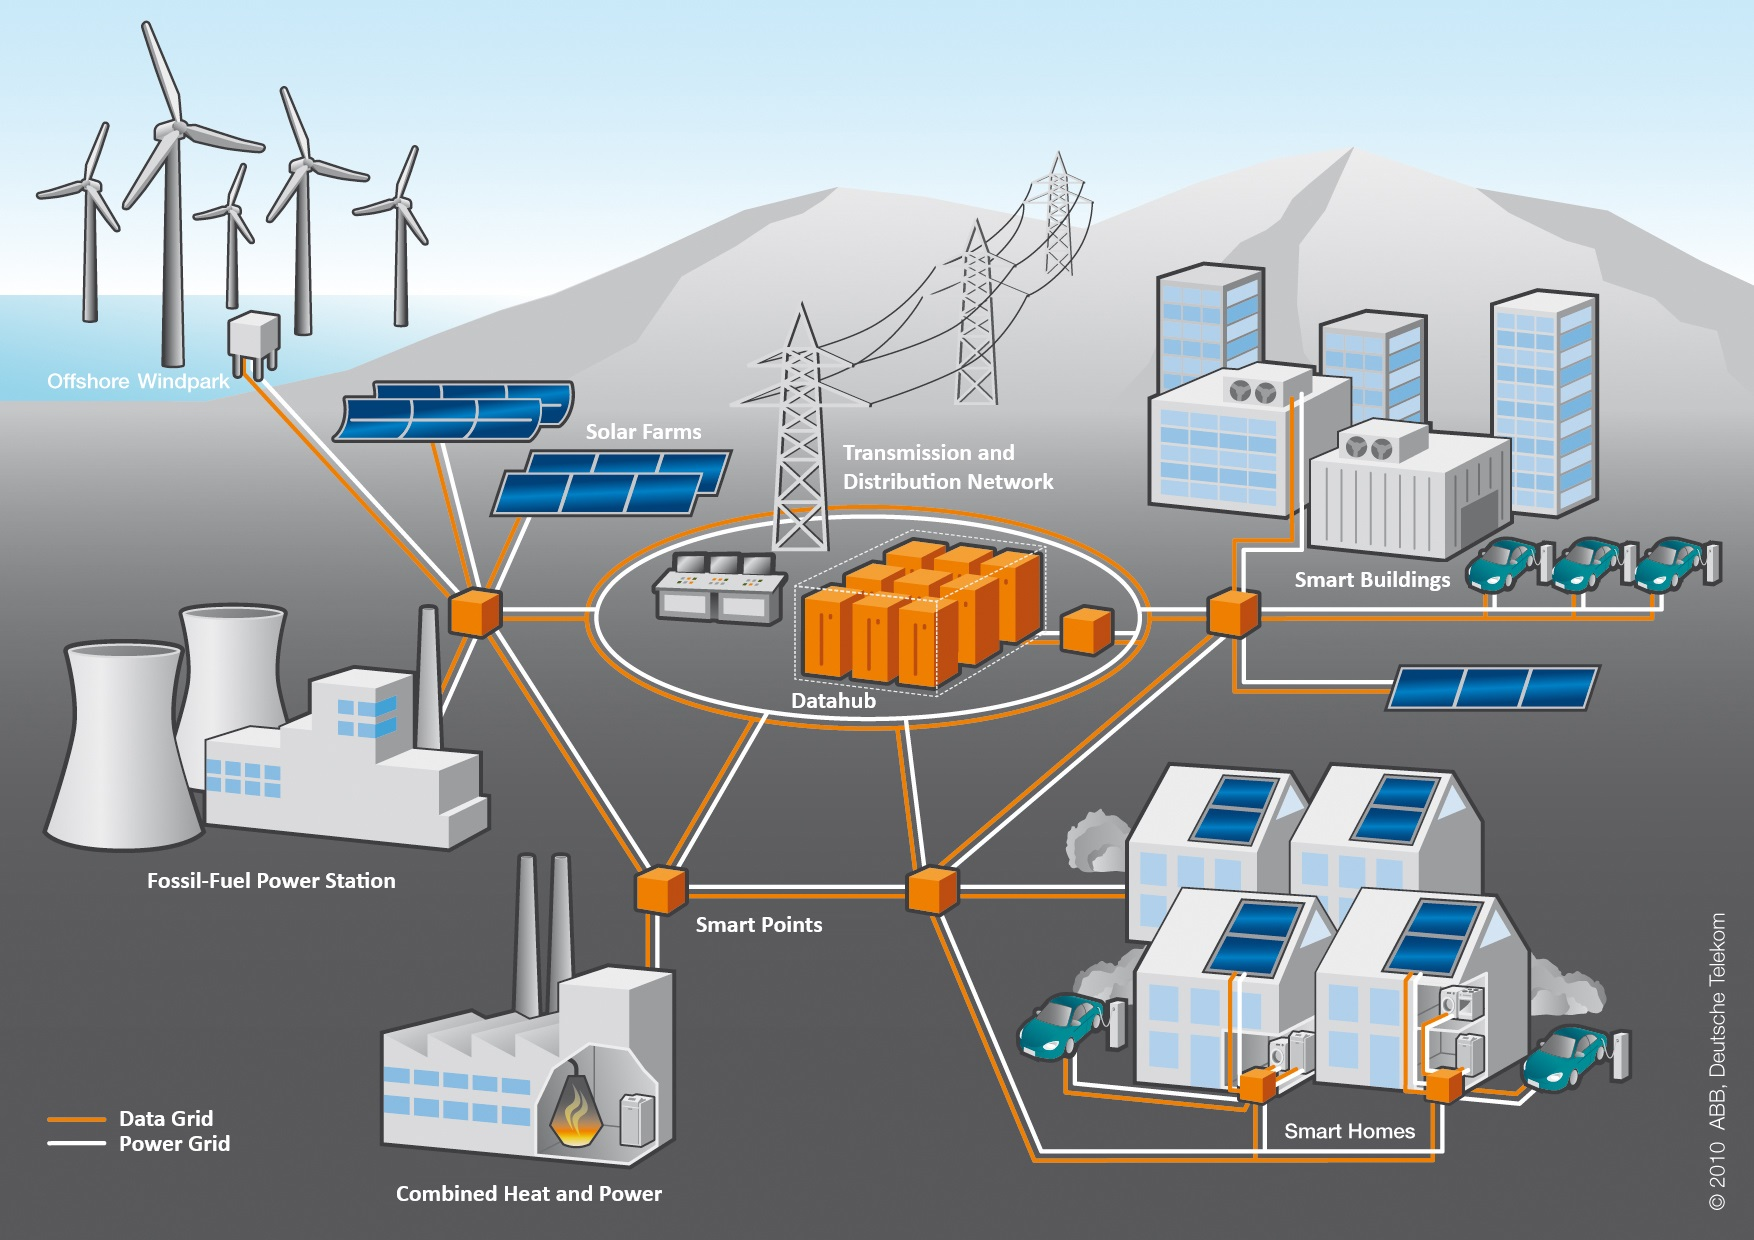
\includegraphics[width=\textwidth]{figures/SmartGrid_Ueberblick_ohneLegende.jpg}
	\caption{\url{http://powertown.no/wp-content/uploads/2011/11/SmartGrid_Ueberblick_ohneLegende.jpg} \url{https://www.telekom.com/medien/bild-ton-und-infografiken/infografiken/155030}
		\mikael[]{This needs to be translated.}
		\mikael[]{Don't know how to handle figure source(s), also in relation to translation.}
	}
	\label{fig:background:smartgrid}
\end{figure}

\subsection{Problems}
In regards to enabling an EU-wide smart grid, there are bound to be problems as this is an immense project.
This roll-out will not be the same in every nation, as each nation has its own infrastructure and differs in which parts of the current power-grid is owned/regulated by state and what is part of a free market.
However, some shared problems still exist, such as privacy, conflict of interest, and attack vulnerabilities \cite{offswitch} \cite{smart_meter_survey}.

\paragraph{Different architectures}

\paragraph{Privacy}

\paragraph{Conflict of interest}

\paragraph{Vulnerabilities}
